\documentclass[12pt]{article}
% The Wrong Unit of Uncertainty — design-aware adaptive conformal inference.
\usepackage[T1]{fontenc}
\usepackage[margin=1in]{geometry}
\usepackage{amsmath,amssymb,amsthm}
\usepackage{graphicx}
\usepackage{booktabs}
\usepackage{natbib}
\usepackage[ruled,vlined]{algorithm2e}
\PassOptionsToPackage{hyphens}{url}  % let the repository URL break at hyphens
\usepackage{hyperref}
\usepackage{xcolor}
\usepackage{setspace}
\doublespacing

\newtheorem{theorem}{Theorem}
\newtheorem{proposition}{Proposition}
\newtheorem{lemma}{Lemma}
\newtheorem{corollary}{Corollary}
\theoremstyle{definition}
\newtheorem{assumption}{Assumption}
\newtheorem{definition}{Definition}
\theoremstyle{remark}
\newtheorem{remark}{Remark}

\graphicspath{{figures/}}
\newcommand{\Ftilde}{\widetilde{F}}
\newcommand{\Gtilde}{\widetilde{G}}
\newcommand{\rhohat}{\widehat{\rho}}
\DeclareMathOperator{\SE}{SE}

\title{The Wrong Unit of Uncertainty:\\
Simultaneous Inference for Repeated Cross-National Surveys}
\author{Kunwoo Park\\
\small Department of Political Science and International Relations,\\
\small Kookmin University, Seoul, Republic of Korea\\
\small \texttt{pkw31386094@gmail.com} \quad ORCID: 0009-0007-9067-8964}
\date{}

\begin{document}
\maketitle

\begin{abstract}
Repeated cross-national surveys are used to make claims about whole
trajectories of national response distributions, while uncertainty is
computed for single wave contrasts. When country trajectories calibrate
cross-country prediction, moreover, the calibration objects are themselves
complex-sample estimates. We develop simultaneous inference that
attaches uncertainty to both units. Within a country, one design-based band
certifies a partially ordered family of trajectory claims, from a single
wave pair to persistent decline across a preregistered core of the
distribution, with no further correction. Across countries, a clustered
conformal band gives finite-sample coverage for survey-estimated
trajectories. We prove that correcting toward the latent trajectory is
unidentified without design-noise information, and characterize when the
correction is unnecessary, not reliably learnable at the available $K$, or
feasible: infeasible across countries, active one unit down. In the
European Social Survey a marginal reading flags twenty of thirty countries;
six certify net decline over 2018--2024, and over 2002--2024 none certifies a
persistent slide, a claim that only crisis-scale change reliably clears,
while closed testing certifies at least six true span decliners among
thirty-three. The same procedure cuts the certified WVS deconsolidation set
severalfold, toward post-communist and Arab-Spring states.
\end{abstract}

\section{Introduction}

Comparative politics increasingly treats a national public as a
\emph{distribution} rather than a mean \citep{dimaggio1996americans}. Trust in parliament in a country and
year is a cumulative distribution function over a response scale, and
repeated cross-national surveys, among them the European Social Survey
\citep[ESS;][]{kaminska2017survey}, the World Values Survey (WVS), and the
AmericasBarometer \citep{lapop2021pulse}, generate claims about how those
distributions evolve across waves. A second use, \emph{transporting} trajectories (predicting one country's
from the others'), draws on conformal prediction's finite-sample,
distribution-free coverage \citep{vovk2005algorithmic,lei2018distribution}
and its shift relaxations
\citep{tibshirani2019conformal,gibbs2021adaptive,gibbs2024conditional}.

\paragraph{Two wrong units.} One principle organizes this paper: \emph{the
stochastic unit of a guarantee must coincide with the unit of the scientific
claim it certifies}
\citep{robinson1950ecological,openshaw1984modifiable}. Claims from repeated
surveys violate it twice.
Uncertainty is routinely reported for a local contrast, one wave pair at one
threshold, while the \emph{claim} it is taken to support (``democratic
trust is declining'') concerns a whole trajectory. The deconsolidation debate
of \citet{foa2016democratic,foa2017signs} and \citet{valgardsson2025crisis}
is the substantive case we re-examine, not a methodological culprit, since
its own evidence is cohort comparisons. The
second, subtler wrong unit is the calibration: the objects conformal
transport calibrates on are themselves \emph{estimated} from complex
probability samples, and existing constructions plug them in as if exact \citep{dunn2023distribution,lee2023distribution}.

The two errors are distinct. Writing $F_{c, r}(t)$ for country $c$'s latent CDF at
threshold $t$ in wave $r$ and $\Ftilde_{c, r}(t)$ for its complex-survey estimate,
\begin{equation}\label{eq:decomp}
\Ftilde_{c, r}(t) - \mu_r(t)
\;=\; \underbrace{\big(F_{c, r}(t)-\mu_r(t)\big)}_{\text{transport error}}
\;+\; \underbrace{\big(\Ftilde_{c, r}(t)-F_{c, r}(t)\big)}_{\text{design error}},
\end{equation}
where $\mu_r$ is the transport center. A band calibrated on the observed
$\Ftilde$ scores treats the sum as if it were the transport error alone. Its
spread mixes cross-population variation with survey-design variation
that is irrelevant to the latent target, so the band can be inefficient
(under a scale family its target scale is inflated by the familiar
$1/\sqrt{1-\rho^2}$). Yet a correction that subtracts the survey noise,
itself estimated from a handful of countries, can make the band too narrow.

\paragraph{Contributions.} We make four.
\emph{First, a procedure for the claim unit}: a design-based simultaneous band
over a country's whole trajectory. From it a partially ordered family of
claims, from a single wave pair up to persistent decline over a
preregistered core of the distribution, is read off one coverage event
(Section~\ref{sec:claims}).
\emph{Second, an identification boundary for the calibration unit.} Without
information on the design-noise law the latent transport-error law is
non-identified, and no band built on the observed curves can uniformly improve
on the plug-in conformal band beyond its discreteness slack while remaining
valid (Theorem~\ref{thm:impossible}).
\emph{Third, the feasibility boundary of the correction, and a selector that
respects it.} Even with the design-noise information supplied, the
correction's reliability diagnostic obeys an algorithmic floor
$D\ge\sqrt{2/(K-1)}$, so the deployed correction requires $K\ge94$
exchangeable populations. The two largest surveys fail this bound in
opposite ways, while one unit down, on regions within countries
($K\approx230$--$290$), the same frozen selector activates
(Section~\ref{sec:evidence}). The anchor band is finite-sample valid at
every $K$, exact under its symmetric centers and carried into the released
leave-one-out deployment by an explicit $K/(K{-}1)$ inflation, and the
selector preserves each branch's guarantee (Theorems~\ref{thm:exact} and~\ref{thm:safe}). The clustered band itself is
machinery shared with a companion paper on a non-survey domain
\citep{park2026poverty}; new here is what the survey layer forces: the identification boundary, the floor, the safe selector, and the
claim-family deployment.
\emph{Fourth, two reanalyses in which the procedures change the substantive
picture} (Section~\ref{sec:political}). For European trust, net decline
certifies in six of thirty countries (2018--2024) against the twenty a
marginal reading flags, and over 2002--2024 no country certifies
persistence while eight certify span erosion, all read off one band per
country. Globally, a trajectory-persistence criterion cuts the Foa--Mounk
``deconsolidation'' set on the WVS trend file (1981--2022) by
$2.6$--$6.5\times$, leaving a thirteen-country descriptive co-certified core;
twelve pass a dependence-robust test of at least two true item declines. The geography remains
post-communist and Arab-Spring-aftermath states.

\section{Setup and the two targets}\label{sec:setup}

\paragraph{Objects.} We observe $K$ source countries, indexed $c=1, \dots, K$,
treated as exchangeable units (the exchangeable object is the country, not the
respondent). Each country has a latent \emph{response-distribution
trajectory} $F_{c, r}(t)$, a CDF over a fixed grid of thresholds
$t\in\{t_1, \dots, t_T\}$ and survey rounds $r$. We say \emph{response
distribution} deliberately: guarantees attach to recorded answers, and reading
a certified shift as an \emph{attitude} shift additionally requires
measurement invariance across waves (Section~\ref{sec:discussion}); one
invariance comes free, since every claim below survives monotone recoding of
the ordinal scale. We do not see $F_{c, r}$; we see a complex-survey estimate
$\Ftilde_{c, r}(t)=F_{c, r}(t)+S_{c, r}(t)$, where $S_{c, r}$ is design (sampling) error
with a design variance $v_{c, r}(t)^2$ that a stratified
primary-sampling-unit (PSU) / replicate-weight bootstrap can estimate. Write
$E_c=\{F_{c,r}(t)-\mu_r(t)\}_{r,t}$ and
$\widetilde E_c=\{\Ftilde_{c,r}(t)-\mu_r(t)\}_{r,t}$ for the latent and
observed deviation curves of~\eqref{eq:decomp}. The transport score of a
country is its worst-case standardized deviation from the transport center,
\[
R_c \;=\; \max_{r, t}\frac{|F_{c, r}(t)-\mu_r(t)|}{\sigma(t)},
\qquad
\widetilde{R}_c \;=\; R_c + \xi_c,
\]
with $\sigma(t)$ a fixed modulation profile (the deployed anchor takes
$\sigma\equiv1$, the unstudentized score), $\widetilde{R}_c$ the same
quantity from the observed $\Ftilde$, and $\xi_c:=\widetilde R_c-R_c$ the
induced design contamination (treating it as centred additive noise is a
working approximation; the impossibility below works at the curve scale
instead). The governing scalar is the design-to-total SD ratio
\[
\rho \;=\; \frac{\text{SD}(\xi)}{\text{SD}(\widetilde R)}
\;=\;\sqrt{\frac{\overline{v^2}}{s_R^2+\overline{v^2}}}\;\in\;[0,1),
\]
with $s_R^2$ the between-country variance of the latent scores and
$\overline{v^2}$ the average design variance: $\rho\to0$ is the
design-noise-negligible regime, $\rho\to1$ the noise-dominated one.

\paragraph{Target and validity.} We want a simultaneous band covering a
new country's \emph{latent} trajectory (target T2),
$\Pr\big(F_{\text{new}, r}(t)\in\widehat B(r, t)\ \forall r, t\big)\ge1-\alpha$;
the \emph{survey-estimate} trajectory $\Ftilde_{\text{new}}$ is target T1.
Ordinary clustered conformal on the observed scores is exact for T1 under
exchangeability and a symmetric center (Theorem~\ref{thm:exact}); its latent
coverage differs by an explicit gap vanishing with
the design-noise scale (Theorem~\ref{thm:oracle}(b); symmetry alone is not
enough), its width is inflated by design noise, and correcting that is a
deconvolution. Table~\ref{tab:targets} collects the paper's
procedure--target--guarantee triples.

\begin{table}[t]
\centering\small
\begin{tabular}{@{}p{0.26\textwidth}p{0.21\textwidth}p{0.22\textwidth}p{0.24\textwidth}@{}}
\toprule
Procedure & Target & Key assumption & Guarantee \\
\midrule
Clustered conformal band (anchor) & survey-estimated trajectory &
  country exchangeability & finite-sample, every $K$, under symmetric centers
  (Thm~\ref{thm:exact}) \\
\addlinespace[2pt]
Same band, latent reading & latent trajectory & + design-noise tail and
  anti-concentration & $1{-}\alpha{-}\mathrm{gap}$, gap shrinking with $\rho$
  (Thm~\ref{thm:oracle}b) \\
\addlinespace[2pt]
Design-aware correction & latent trajectory & design law (A1)--(A3),
  $K\ge94$ & $1{-}\alpha{-}\varepsilon_{K,B}$; deployed level a frozen
  calibrated bound (Thm~\ref{thm:estimated}) \\
\addlinespace[2pt]
Certification band (\S\ref{sec:claims}) & within-country contrast surface &
  survey-design bootstrap & asymptotic simultaneous $1{-}\alpha$ \\
\bottomrule
\end{tabular}
\caption{Which procedure guarantees what. The conservative envelope (omitted)
shares the anchor's row, containing it by construction; the theory's
finite-sample language does not transfer to the certification
band.}\label{tab:targets}
\end{table}

\paragraph{What country exchangeability assumes.} The transport band's
identifying assumption is a superpopulation postulate: participating countries'
trajectory laws are symmetric draws, over a set that is not sampled and enters
rounds non-randomly --- a strong idealization, tempered three ways: the
headline certifications of Section~\ref{sec:political} do not use it; under
approximate exchangeability the \citet{barber2023conformal} bound controls the
gap; and a leave-one-region-out audit finds near-nominal held-out coverage
except for the post-communist East (Supplementary Material).

\paragraph{The impossibility.} The central obstruction is that the deconvolution
is not identified from the contaminated curves alone. The result is stated at
the curve level of~\eqref{eq:decomp}, where the additive model \emph{is} the
survey sampling structure; the design noise may be arbitrarily heteroskedastic
across thresholds.

\begin{theorem}[Non-identification and necessity of design information]
\label{thm:impossible}
Let the observed deviation curves be $\widetilde E_c = E_c + S_c$ as
in~\eqref{eq:decomp}, the latent curves exchangeable with law $\mathcal L_E$,
the design-noise curves independent of them with law $\mathcal S$ in an
admissible class that contains $S\equiv0$ and is closed under one further
nondegenerate symmetric convolution. (i)~$\mathcal L_E$ is not identified from
the observed law $\mathcal L_E*\mathcal S$. (ii)~Any band whose radius is
measurable in the observed curves alone and is valid for the latent target
over the whole admissible class cannot uniformly improve on the plug-in
conformal band: on the member $S\equiv0$, which it cannot distinguish from the
contaminated configurations, the plug-in radius is already the tightest valid
one up to the conformal discreteness slack, which randomized smoothing
exhausts. Uniform improvement requires shrinking the class of noise laws.
\end{theorem}

The reading is constructive (proof in the Supplementary Material, Section~S1):
a band both valid and narrower than the plug-in must supply the design-noise
law --- exactly what Section~\ref{sec:method}'s design bootstrap does.

\begin{remark}[Beyond surveys]\label{rem:general}
Nothing here is survey-specific: the result holds whenever conformal calibration
uses estimated objects --- model-based small-area outputs, learned or imputed
features, meta-analytic effects. Design/measurement information is the
identifying ingredient, and its reliability at finite $K$ is itself bounded
(Proposition~\ref{prop:unreach}); confirmed on a non-survey small-area
calibration in simulation (Supplementary Material).
\end{remark}

\paragraph{Relation to existing work.} Conformal prediction has met complex
surveys for unit-level prediction \citep{wieczorek2023design}, and
cluster-as-unit constructions transport guarantees to an unseen cluster while
treating its data as cleanly sampled
\citep{dunn2023distribution,lee2023distribution}; our calibration objects are
instead estimated under complex designs
\citep{binder1983variances,lumley2010complex}. Noise-aware conformal methods
correct under a \emph{known} noise model
\citep{einbinder2024label,sesia2025adaptive,singer2025conformal};
Theorem~\ref{thm:impossible} says that premise fails for design noise --- a
deconvolution problem \citep{fan1991optimal} --- and
Proposition~\ref{prop:unreach} that even a supplied law faces a finite-$K$
floor.

\section{Simultaneous inference for both units}\label{sec:method}

The two wrong units get two procedures: within-country certification of a
whole claim family, and cross-country transport with a correction that
activates only where it is provably reliable.

\subsection{Within-country certification: one band, a family of claims}
\label{sec:claims}

The claims of interest differ in their unit. A \emph{pairwise} claim asks
whether a given adjacent pair of waves shows a distributional shift;
\emph{any-pair} whether some adjacent pair does; \emph{net} whether the
first-to-last span declined; \emph{persistent country-wide} whether the whole
distribution declined simultaneously across the trajectory; \emph{Bonferroni}
further controls the number of countries examined. These claims form a partial
order, not a chain: persistent implies both net and any-pair, but net and
any-pair are incomparable --- a dip that recovers certifies an adjacent pair
with no net decline, and a slow accumulation can certify a long span while no
single adjacent pair clears the critical value; both patterns occur in the ESS
record (Section~\ref{sec:political}). The claims are not separate tests: each
claim, every sub-span, and the reverse direction is a function of one object,
the country's surface of wave-pair contrasts, so all are certified on one
coverage event. Reading one claim as another is the over-detection this paper
is about.

\begin{proposition}[Claim-family transfer]\label{prop:transfer}
Let $\widehat B$ be a simultaneous $1-\alpha$ band for a country's contrast
surface $\theta=\{\theta_{a, b}(t)\}$ over every ordered pair of observed rounds,
and let $\{A_j\}$ be any family of claims, each a set of surfaces. Define
the certified subfamily $J=\{j: \widehat B\subseteq A_j\}$. Then
$\Pr\big(\theta\in A_j\ \text{for every}\ j\in J\big)\ge1-\alpha$, with no
dependence on $|J|$: on $\{\theta\in\widehat B\}$, set inclusion delivers every
certified claim at once.
\end{proposition}

The proof is the line just given; reading each deterministic consequence off
one simultaneous region is the post-hoc logic of \citet{scheffe1953method},
closed testing \citep{marcus1976closed}, and the selection-free bounds of
\citet{goeman2011multiple,katsevich2020simultaneous}. The contribution is its
deployment: trend claims in this literature are made claim by claim, and one
studentized sup-$t$ band over the whole contrast family removes the
corrections a per-claim construction needs --- no Bonferroni across a
country's pairs, no separate budget for certified recoveries, no
endpoint-selection cost --- at the price of a wider critical value, which we
report. The persistent object is covered directly by one functional band
\citep{diquigiovanni2021conformal}, a distinction of estimand rather than
error rate \citep{gelman2012why,benjamini1995controlling}. The band itself is
a design-based simultaneous sup-$t$ band on wave-pair CDF differences from the
stratified-PSU bootstrap \citep{rao1988resampling,wolter2007introduction}: an
asymptotic guarantee in which exchangeability plays no role, and to which the
theory sections' finite-sample language does not transfer.

\subsection{Cross-country transport and the safe adaptive band}
\label{sec:transport}

Theorem~\ref{thm:impossible} says the design bootstrap is the identifying
input; the transport method turns it into a band by choosing, target-blind,
among three constructions.

\paragraph{Three branches.} For calibration error curves $\{\widetilde E_c\}_{c=1}^K$
over threshold grid $t$, with per-country design SD $\widehat v_c(t)$ from the
stratified-PSU bootstrap:
\emph{(i) The clustered conformal band} takes the conformal quantile of the
\emph{unstudentized} scores $\max_t|\widetilde E_c(t)|$: exact for the
survey-estimate target at any $K$ under Theorem~\ref{thm:exact}'s symmetric
centers, with the latent gap of Theorem~\ref{thm:oracle}(b).
\emph{(ii) Deconvolution} studentizes by the finite-$K$-guarded target scale
$\widehat s_{T}^2(t)=\max\!\big(s_{\text{plug}}^2(t)-[\, \overline{\widehat v^2}(t)-z\, \SE\, ]_+, \ \text{floor}\big)$,
which subtracts a \emph{lower} confidence bound on the design variance so the
correction cannot over-shrink; its width scales as $\sqrt{1-\rho^2}$ relative to
the clustered band. \emph{(iii) Conservative} inflates each unstudentized score by the design SD,
$\max_t(|\widetilde E_c(t)|+z\, \widehat v_c(t))$, a score that dominates the clustered
band's score pointwise, so the conservative band \emph{contains} the clustered
band by construction.

\paragraph{Safe selector (Algorithm~\ref{alg:safe}).} A naive selector asks
\emph{can we deconvolve} and \emph{do we need to}; the safe selector adds the
missing third question, \emph{can we do it safely at this $K$?} Deconvolution
is used only when four gates pass, all computed from the calibration set
alone: \emph{need} (A: $\rhohat_{\text{LCB}}>\rho_0$, a conservative lower
confidence bound on $\rho$), \emph{reliability}
(B: $\widehat\delta_{\text{UCB}}(D)\le\delta_{\max}$, a frozen upper confidence
bound on the finite-$K$ coverage remainder through the diagnostic
$D=\max_t \SE(\widehat s_T^2)/\widehat s_T^2$), \emph{efficiency}
(C: a certified width gain $\widehat{\text{Gain}}$ over the conservative band
clearing a margined threshold), and \emph{stability} (D); otherwise the band
is an anchor, as Algorithm~\ref{alg:safe} routes. Every gate is target-blind, so by
Theorem~\ref{thm:safe}'s nested-band argument validity survives even
adversarial selection between the anchor branches; the non-nested
deconvolution branch is charged its own miss budget, and only in the $K\ge94$
regime where its gate can open at all (Section~\ref{sec:theory}). All
constants are frozen before validation (Supplementary Material); when
deconvolution is used the reported level is the observable
$1-\alpha-\widehat\delta_{\text{UCB}}(D)$, a frozen \emph{calibrated} bound
(the theorem-level guarantee is Theorem~\ref{thm:estimated}'s
$\varepsilon_{K, B}$). The method ships as one call,
\texttt{dapcb(cal\_errors, v\_cal, center, alpha)}, returning the band, the
selected branch and why, the coverage level, and the target that level refers
to.

\begin{algorithm}[t]
\caption{Nominal-safe adaptive design-aware band}\label{alg:safe}
\KwIn{calibration curves $\{\widetilde R_c\}$ (unit = country), design replicates
$\{\widehat v_c\}$, target curve $\widehat F_{\text{new}}$, level $\alpha$;
frozen gate constants and the $K$-only budget rule $\alpha_{\text{dec}}(K)$}
set $(\alpha_{\text{anchor}}, \alpha_{\text{dec}})$ by the frozen budget rule
(full $\alpha$ to the anchors when gate B is infeasible at this $K$)\;
compute diagnostics $s$, $\widehat s_T$, $\rhohat_{\text{LCB}}, D,
\widehat\delta_{\text{UCB}}(D)$; the nested unstudentized anchor radii
$r_{\text{clu}}, r_{\text{con}}$ at level $\alpha_{\text{anchor}}$; and
$r_{\text{dec}}$ at level $\alpha_{\text{dec}}$\;
\uIf{$\rhohat_{\text{LCB}}\le\rho_0$}{branch $\leftarrow$ clustered\;}
\uElseIf{$\widehat\delta_{\text{UCB}}(D)\le\delta_{\max}$ \textbf{and} stable
\textbf{and} $\widehat{\text{Gain}}-\Delta_g>g_{\min}$}{branch $\leftarrow$
deconvolution\;}
\Else{branch $\leftarrow$ conservative\;}
\If{\upshape branch $\neq$ deconvolution \textbf{and} the center is
leave-one-out (the unsurveyed-target default)}{
$r_{\text{branch}}\leftarrow\frac{K}{K-1}\,r_{\text{branch}}$
\tcp*{exactness for the deployed center (Section~\ref{sec:theory})}}
\Return $\widehat F_{\text{new}}\pm r_{\text{branch}}$, branch, and diagnostics\;
\end{algorithm}

\section{Theory}\label{sec:theory}

Table~\ref{tab:targets} maps each procedure to the target it covers. Proofs
are in the Supplementary Material, Section~S1.

\begin{theorem}[Oracle validity]\label{thm:oracle}
Suppose the countries are exchangeable and the design law is known.
(a)~The clustered band is finite-sample valid for the survey-estimate target,
$\Pr(\Ftilde_{\text{new}}\in\widehat B)\ge1-\alpha$, using exchangeability only.
(b)~For the latent target the same band satisfies, for every $u>0$,
$\Pr(F_{\text{new}}\in\widehat B)\ge1-\alpha-\Pr(\xi<-u)-
\Pr(\widetilde R\in(\widehat q-u,\widehat q\,])$.
(c)~Under the scale-family condition (A1), the oracle deconvolution band
with the true target scale is finite-sample valid for the latent target and
exact at the attainable conformal rank, and its target scale is a factor
$\sqrt{1-\rho(t)^2}$ of the observed scale at each coordinate. The realized
width carries, in addition, the ratio of the two conformal quantiles, which
tends to one as $\rho\to0$. Some such shape restriction is necessary
(Supplementary Material).
\end{theorem}

The gap in~(b), a noise-tail term plus a local anti-concentration term,
vanishes with the design-noise scale (order $\sigma_\xi^{2/3}$ under
variance-only tails, $\sigma_\xi$ up to logarithms under sub-Gaussian
noise, $\sigma_\xi$ a scale for $\xi$) but not by symmetry alone (a bimodal
counterexample is in the Supplementary Material). Hence we estimate and
report the design share rather than assume it away.

\begin{theorem}[Exact finite-$K$ validity of the deployed base band]\label{thm:exact}
Let the base band use the unstudentized cluster score of the \emph{observed}
curves, $\widetilde R_c=\max_t|\Gtilde_c(t)|$ ($t$ ranging over the
stacked round-by-threshold grid; the latent $R_c$ of
Section~\ref{sec:setup} is unobserved), with a center satisfying the
symmetric-construction condition (the Supplementary Material states the four
admissible cases). If the countries are exchangeable, then for every $K$ the
band $\widehat B=\text{center}\pm\widehat q$, with $\widehat q$ the
$\lceil(1-\alpha)(K{+}1)\rceil$-th order statistic of
$\{\widetilde R_c\}_{c\le K}$ (and $\widehat q=\infty$ when that rank
exceeds $K$, i.e.\ when $K<\alpha^{-1}-1$), satisfies
$\Pr(\Ftilde_{\text{new}}\in\widehat B)\ge\lceil(1-\alpha)(K{+}1)\rceil/(K{+}1)\ge1-\alpha$,
distribution-free, with equality at the stated rank level when the scores are
almost surely distinct. The guarantee holds at every $K$; the band is
informative only for $K\ge\alpha^{-1}-1$.
\end{theorem}

Exactness at every $K$ is bought by excluding two asymmetries, in-sample
modulation and grand-mean centers that contain their own unit, at a width
cost of at most $5\%$ on the near-homoskedastic real curves.

\begin{theorem}[Estimated-law validity]\label{thm:estimated}
Assume a common scale family indexed by the design variance (A1),
anti-concentration of the sup-score law near its upper quantile (A2), and
bounded curves with a size-$B$ design bootstrap whose ideal variance is the
design variance (A3), stated in full in the Supplementary Material with the
bootstrap's two layers separated. Then (i)~with oracle scales the deconvolution band
is finite-sample valid for the latent target at every $K$ and exact at the
attainable conformal rank, and (ii)~with
estimated scales it satisfies
$\Pr(F_{\text{new}}\in\widehat B)\ge 1-\alpha-\varepsilon_{K,B}$ with
$\varepsilon_{K,B}=O\big(\sqrt{\log(KT)/\min(K,B)}\,\big)$.
\end{theorem}

By construction the finite-$K$-guarded scale
$\widehat s_T^2$ of Section~\ref{sec:method} subtracts a one-sided margin
below the mean design variance, so on the guard event (Supplementary
Material) the design-variance-subtraction component of the scale error can
only widen the band. The sampling error in $s_{\mathrm{plug}}^2$ stays
two-sided and is absorbed into $\varepsilon_{K,B}$. (A1) matches the
\emph{distributions} of standardized observed and latent curves, more than
equal covariance profiles give; Gaussian families satisfy it. The
survey-scale guarantee does not rest on it: where it is doubtful the selector
abstains.

The two clauses below cover different targets: the survey-estimated
trajectory below the floor, the latent one above it.

\begin{theorem}[Safe-adaptive finite-$K$ validity]\label{thm:safe}
Let the anchors use Theorem~\ref{thm:exact}'s centers (or the leave-one-out
center with its $K/(K{-}1)$ inflation, Propositions~S1 and~S3). For the
first clause assume the countries' observed trajectories exchangeable; for
the second assume (A1)--(A3). Deploy Algorithm~\ref{alg:safe} with the
unstudentized clustered and conservative branches, scores
$\max_t|\Gtilde_c(t)|$ and $\max_t(|\Gtilde_c(t)|+z\widehat v_c(t))$,
at level $\alpha_{\text{anchor}}$,
and the deconvolution branch at $\alpha_{\text{dec}}$. Then, with no
condition on the selection rule,
\begin{gather*}
\Pr\big(\Ftilde_{\text{new},r}(t)\in\widehat B(r,t)\ \forall r,t\big)\ge1-\alpha\ \ (K<94),\\
\Pr\big(F_{\text{new},r}(t)\in\widehat B(r,t)\ \forall r,t\big)\ge1-\alpha-\varepsilon_{K,B}\ \
(K\ge94),
\end{gather*}
the first clause finite-sample, the second carrying
Theorem~\ref{thm:estimated}'s remainder.
\end{theorem}

\emph{Proof sketch.} Below the floor gate~B cannot open
(Proposition~\ref{prop:unreach}(b) is a deterministic identity of the frozen
diagnostic), so the selector only ever chooses between the two anchors. Their scores are ordered pointwise,
$|\Gtilde_c(t)|+z\widehat v_c(t)\ge|\Gtilde_c(t)|$, so at a common level the
conservative order statistic is at least the clustered one and the bands are
nested, $\widehat B_{\text{clu}}\subseteq\widehat B_{\text{con}}$. A miss of
whichever band is selected implies a miss of $\widehat B_{\text{clu}}$,
which Theorem~\ref{thm:exact} bounds by $\alpha$. This is the first clause;
it conditions on no selection event
\citep{gupta2022nested,yang2024selection}. At $K\ge94$ the budget splits,
$\alpha=\alpha_{\text{anchor}}+\alpha_{\text{dec}}$, by a frozen rule of $K$
alone. Under (A1) each
observed calibration score dominates its latent counterpart, since
$\sqrt{s_R^2+v_c^2}\ge s_R$ pointwise, so the anchor quantile
stochastically dominates the latent-score order statistic, and the anchors
are valid for the \emph{latent} target at $\alpha_{\text{anchor}}$
(anchor-domination lemma, Supplementary Material). With the deployed
leave-one-out center they pay a same-order centering term
(Proposition~S3), absorbed into $\varepsilon_{K,B}$. The non-nested
deconvolution branch is charged its own budget by a union bound,
$\Pr(\text{miss})\le\Pr(\text{miss},\widehat J\ne\text{dec})+
\Pr(\text{miss},\widehat J=\text{dec})\le\alpha_{\text{anchor}}+
\alpha_{\text{dec}}+\varepsilon_{K,B}$, the last term from
Theorem~\ref{thm:estimated}(ii) for the always-deconvolve band, its own
centering term priced the same way (Supplementary Material). No term
conditions on $\widehat J$.

A scope note. The unsurveyed-target deployment uses a leave-one-out center,
outside Theorem~\ref{thm:exact}'s symmetric constructions, but inflating the
radius by $K/(K{-}1)$ restores finite-sample validity at every $K$,
distribution-free (Proposition~S1). The released default ships that
inflation at a width cost of $1/(K{-}1)$, $3.5\%$ at the ESS's
$K\approx30$. The exact split-fold alternative is infeasible at survey scale:
halving the calibration set below $\alpha^{-1}{-}1$ units makes the
conformal radius infinite.

\paragraph{Efficiency.} Under (A1) the deconvolution band reduces
continuously to the clustered band as $\rho\to0$, with oracle scale factor
$\sqrt{1-\rho(t)^2}=1-\tfrac12\rho(t)^2+O(\rho(t)^4)$ at each coordinate;
the conservative band contains the clustered one pointwise; and selection
cannot inflate miscoverage (Theorem~\ref{thm:safe}).

\section{Simulation}\label{sec:simulation}

Simulation establishes two facts: the wrong unit collapses coverage, and
the safe selector meets its guarantees on unseen data.

\subsection{The wrong unit collapses coverage}\label{sec:wrongunit-sim}

We simulate $K=30$ countries and $T=6$ thresholds over trajectories of
length $L$ rounds, with errors correlated across rounds and thresholds, and
ask each band for \emph{trajectory} coverage
(Figure~\ref{fig:wrongunit}). All three bands are unstudentized and
finite-sample, so only the score's unit varies. A band that is marginally
valid at the round level covers the trajectory $81.7\%$ of the time at $L=2$
and $49.8\%$ at $L=8$; per threshold the figures are $38.2\%$ and $3.5\%$.
Only the country-trajectory band holds its nominal $90\%$ at every length,
because the trajectory is a single exchangeable unit. The obvious rejoinder, correcting the wrong-unit bands for multiplicity,
fails at survey scale. A Bonferroni-corrected per-round band needs a conformal quantile at
level $\alpha/L$, which exists only for $K\ge L/\alpha-1$ countries ($79$ at
$L=8$; $479$ for the threshold-level band), so at $K=30$ its radius is
infinite for every $L\ge4$. Where it does exist ($K=100$), it is
$4$--$26\%$ wider than the trajectory band for comparable or higher
coverage ($90$--$94\%$ against $89$--$91\%$). The choice is therefore not whether
to correct but which unit carries the simultaneous statement at the $K$
surveys have. The
multiplicity-corrected baselines are a post-preregistration robustness
benchmark.

\begin{figure}[t]\centering
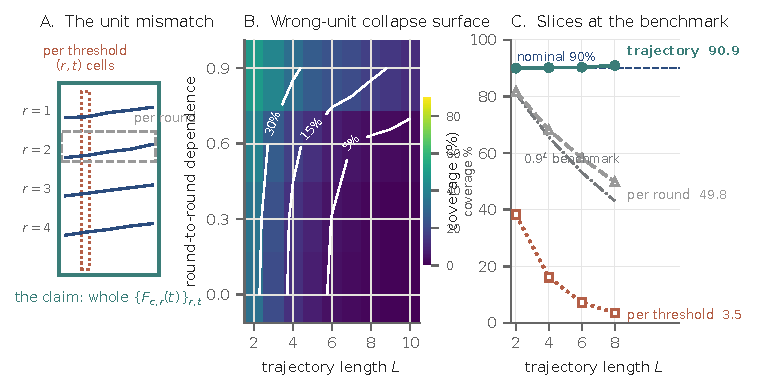
\includegraphics[width=.8\textwidth]{wrong_unit_coverage.pdf}
\caption{Coverage of a whole country trajectory, by the unit the score is
attached to ($4{,}000$ replicates, nominal $90\%$; bars are $\pm2$ Monte Carlo
SEs). Only the trajectory-unit band holds its level as the trajectory
lengthens.}\label{fig:wrongunit}
\end{figure}

\paragraph{Severity: what each claim can detect.} At ESS-like design noise,
$80\%$ power at the \emph{net} claim needs a per-pair decline of $0.02$--$0.03$
CDF points. The \emph{persistent} claim needs $0.06$--$0.08$, a
crisis-scale change, and its power \emph{falls} as the trajectory
lengthens. Injecting known declines into the real ESS pairs puts the
thresholds at $\approx0.033$ (net) and $\approx0.075$ (persistent), with
realized size $0.001$--$0.007$ against a nominal $0.10$. The procedure is
markedly conservative, so non-certification is weak evidence of absence at
every claim. The powered claim for secular decline is the net span
(Section~\ref{sec:political}).

\paragraph{Validation.} The frozen procedure was then evaluated on a sealed
set of six unseen data-generating families, with the script hash recorded
before first execution. All $120$ cells were compatible with the target
coverage (worst $0.878$), with zero activations below $K=94$, as the floor
requires. The three-layer validation history (including a first
holdout demoted to development after a scorer audit) is in the
Supplementary Material.


\section{Evidence from the ESS and the AmericasBarometer}\label{sec:evidence}

\paragraph{The regime characterization.} At the cross-national unit the
selector reduces to the clustered conformal band, not by assumption but by
its own low-$\rho$ gate: across both surveys and every estimand examined,
$\rhohat\le0.22$ on the AmericasBarometer and at most
$0.29$ in the ESS subgroup scan, well below the frozen need cutoff
$\rho_0=0.47$. Every
$\rhohat$ we report is a downward-biased \emph{floor} in expectation, the PSU
bootstrap resampling $m$-of-$m$ without Rao--Wu--Yue rescaling
\citep{rao1992recent}; the rescaled rerun leaves the regime unchanged ---
maxima $0.28$ and $0.22$, zero gate activations, every certification count
unchanged (Supplementary Material).

\paragraph{Why the deconvolution is unreachable, precisely.}

\begin{proposition}[Finite-$K$ feasibility of the deployed correction]\label{prop:unreach}
The deployed selector activates deconvolution only if a \emph{need} gate
$\rhohat_{\mathrm{LCB}}>\rho_0$ and a \emph{reliability} gate $D\le\tau_D$ both
hold, with $D=\max_t \widehat{\mathrm{SE}}(\widehat s_T^2)/\widehat s_T^2$ and
the frozen
$\widehat{\mathrm{SE}}(\widehat s_T^2)=
\sqrt{2s_{\mathrm{plug}}^4/(K{-}1)+(\mathrm{SD}_K(\widehat v^2)/\sqrt K)^2}$.
Both gates are bounded by \emph{algorithmic identities of the frozen
procedure}.
(a) $\rho(t)^2=\overline{v^2}(t)/s_{\mathrm{plug}}^2(t)\in[0,1)$
coordinate-wise, and $\rhohat_{\mathrm{LCB}}$ is its conservative aggregate:
the need gate fires only when design noise is an appreciable fraction of the
between-population spread, $\rho_0$ being a frozen operational threshold.
(b) Since $\widehat s_T\le s_{\mathrm{plug}}$ by construction,
$D\ge\sqrt{2/(K-1)}$, so the reliability gate requires $K\ge1+2/\tau_D^2$, i.e.\
$K\ge94$ at the frozen $\tau_D=0.147$. (The Supplementary Material separates
the deterministic statement from its kurtosis-dependent interpretation.)
\end{proposition}

The two requirements pull apart on real surveys (Figure~\ref{fig:frontier}).
On the ESS the noisiest subpopulations raise $\rhohat$ only to $0.29$ while
$K\le33$ leaves $D\ge0.25$: neither gate opens ($42$ cells, zero
activations). The WVS is the mirror image: its full item-coverage sets
($K=95$--$105$) make the reliability gate feasible, the certification samples
($K=59$--$77$) do not, and either way $\rhohat_{\mathrm{LCB}}\le0.10$ fails
the need gate. The survey large enough to estimate the deconvolution has
almost no design noise to remove; the survey with real clustered noise has
far too few countries. Nor is the floor an artifact of our thresholds: any
\emph{unbiased} variance estimator from $K$ exchangeable populations has
relative standard error at least $\sqrt{2/(K-1)}$ at the Gaussian member
(Lehmann--Scheff\'e; Supplementary Material), so any correction demanding
relative reliability $\tau$ from such an estimate needs $K\ge1+2/\tau^2$ ---
the frozen $\tau_D$ is one instantiation, $94$ its intercept,
$\sqrt{2/(K-1)}$ the law for this estimator class. With the proved width gain
$1-\sqrt{1-\rho^2}$, the $(K,\rho)$ plane splits into three regimes ---
correction \emph{unnecessary}, \emph{unlearnable} (within the
unbiased-variance class), \emph{feasible} --- and this paper's datasets
occupy the three corners.

\paragraph{Where the correction does live: small areas, on this same survey.}
The barrier is about the unit, and the ESS contains a finer one: a region's
departure from its own \emph{national} distribution,
$D_g=F_g-F_{\text{nation}}$, with the transport band calibrated across
regions and the design SD of the difference from one stratified-PSU
bootstrap of the whole country (Supplementary Material). There the design
share is not marginal --- $\rhohat_{\text{LCB}}$ runs $0.26$--$0.52$ and
clears $\rho_0$ in eight of twenty-three \emph{unit-rounds} (minimum
unit size $\times$ round) --- and both gates open
once $K\gtrsim230$: units of forty to sixty respondents, rounds 9 and 10,
$K=228$--$287$. There the \emph{frozen} selector activates the design-aware
branch for the first time on real survey data, a feasibility demonstration
rather than a validation of latent-target coverage (the latent departure is
unobserved): a band $21$--$27\%$ narrower than the conservative envelope at
its validated operational level $0.88$, with certified width-gain lower
bounds of $0.16$--$0.22$ across twelve independent bootstrap streams. The
activation survives the Rao--Wu--Yue rescaled bootstrap, though the
activating cells fall from four to one (Supplementary Material).

The regions nest in twenty-seven countries, nine each, so the objection this
paper would itself raise is that the effective unit is the country. Holding
out whole countries is the diagnostic: calibrating on the other twenty-six
countries' regions leaves the plug-in anchor at $0.89$--$0.90$ against its
$0.90$ target in all twelve cells, within $0.015$ of leave-one-region-out
calibration. Coverage \emph{conditional} on the country does not transfer
(worst held-out countries $0.53$--$0.63$): the guarantee is marginal over
regions and presumes their exchangeability, which shared national dependence
can violate --- the diagnostic bounds that concern, it does not remove it.
In the activating cells the selected band covers $0.93$--$0.98$ against its
$0.88$ on the observed departure, latent-target validity resting on (A1) as
everywhere in that branch. Two scope conditions: reaching $K\gtrsim230$
pools regions coded at different NUTS levels (among the fourteen countries
sharing one level the need gate opens but $K\le140$ keeps the reliability
gate shut), and round 11 never activates (Supplementary Material). The
correction is thus reachable in principle and unreachable across countries:
it lives at the small-area scale, where Theorem~\ref{thm:impossible}'s
remark said it would.

\begin{figure}[t]\centering
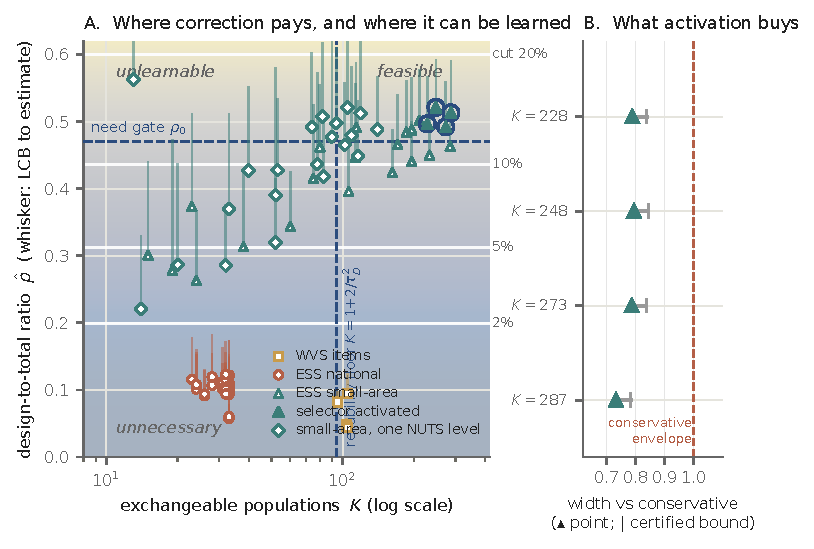
\includegraphics[width=.92\textwidth]{feasibility_frontier.pdf}
\caption{The feasibility frontier in the $(K,\hat\rho)$ plane. Each marker is
a real-data cell at its lower confidence bound, with a bar to the point
estimate; filled markers are the four cells where the frozen selector
activated. Dashed rules are the frozen boundaries, the need cutoff $\rho_0$
and the reliability floor $K=94$.}\label{fig:frontier}
\end{figure}

\section{Political reanalysis: how many democracies really declined?}\label{sec:political}

We analyze trust in parliament (\texttt{trstprl}) and satisfaction with democracy
(\texttt{stfdem}) in ESS rounds 9--11 (2018--2024, the window whose integrated
files ship PSU/stratum identifiers), then extend every trajectory to the full
record (rounds 1--11, 2002--2024), asking, claim by claim, how many countries
survive.
The comparative literature has grown skeptical of a continent-wide trust decline
\citep{norris2017western,voeten2017people,wuttke2022europeans}; we add a
formal procedure that says so and a diagnosis of why the over-reading arises:
the dominant trend estimates \citep{valgardsson2025crisis} rest on
latent-trait models with no design-based uncertainty layer
\citep{taihusolt2024}, and latent-mood estimation
\citep{claassen2019estimating,claassen2020support,kolczynska2026trust} pools
countries into model-based credible intervals, where our bands give
model-free coverage at a stated claim; the two are complements.
Certification levels here are design-bootstrap simultaneous levels,
asymptotic in the within-country samples (Table~\ref{tab:targets}).

\paragraph{The counts collapse across claims.} For \texttt{trstprl} over rounds
9--11, a marginal pairwise reading flags $20$ of $30$
countries; an any-pair
design-aware band drops this to $12$; net first-to-last decline holds in $6$
(Austria, Belgium, Estonia, the United Kingdom, Greece, the Netherlands); and the
\emph{persistent, design-aware simultaneous} band over the preregistered low-trust
core certifies one, Greece, which also survives Bonferroni across countries.
\emph{Greece fielded only rounds 10 and 11 here}, so its trajectory is a single pair and the top claims coincide for it
(as for Czechia and Israel, uncertified). Among the $27$ two-pair
countries none certifies persistence, while the United Kingdom, Belgium, and
the Netherlands pass the \emph{plug-in} persistent claim and are demoted by
the design-aware layer alone. The headline is therefore two numbers: net
decline in six of thirty, and \emph{zero} of the twenty-seven countries
observed across multiple pairs certifying persistence. The severity analysis
(Section~\ref{sec:simulation}) explains why: the persistent claim has $80\%$ power
only against crisis-scale declines, so its non-certifications are weak evidence of
absence. For \texttt{stfdem} the pattern repeats ($23$ marginal, $14$ any-pair,
$8$ net, one persistent: Greece, again one pair, failing Bonferroni there).
The literature reads Greece as a crisis-era legitimacy collapse
\citep{armingeon2014democracy,torcal2014decline}, but those accounts concern
2009--2015 while the certified pair is 2020/21$\to$2023/24.

\paragraph{The long window: the secular question, asked properly.} Extending every
trajectory to its full record (rounds 1--11; median six pairs, up to ten;
rounds 1--8 weights-only in the integrated files; merging their sample-design
files changes no net or persistent count below --- Supplementary Material)
reframes the twenty-year narrative in both directions. Zero of the thirty-three countries with three or more usable rounds
certify persistent decline over the preregistered core across their full
record, plug-in included. Reversing the inequality certifies
\emph{recoveries}, and across the $1{,}173$ ordered contrasts of the trust series
certified movement is directionally balanced ($193$ declining against $212$
rising). Inside the same band, at the same $\alpha$, twenty-three of
thirty-three countries certify at least one decline and at least one
recovery on each outcome (twenty on both); the two directions share one
critical value, so no within-country correction is needed. The count across countries is a
conjunction of thirty-three coverage events and carries no familywise control
by itself; the closed-testing bound below supplies it. The certified record
therefore argues against describing European trust as a uniformly monotone
slide --- on the positive evidence of coexisting certified declines and
recoveries, not on the persistent rung's non-certifications, which its
severity makes weak evidence of absence.

Under Proposition~\ref{prop:transfer}---one band, every ordered contrast and
both directions at $\alpha=0.10$ jointly---net erosion over the
whole span certifies in eight countries (Cyprus, Spain, the United
Kingdom, Greece, Hungary, Israel, Italy, Ukraine;
Figure~\ref{fig:bounds}, Table~\ref{tab:magnitudes}).
Against the per-claim construction the joint statement costs France at the span
claim ($9\to8$) and six countries at the any-pair claim ($28\to22$); the
persistent zero holds under both constructions (Supplementary Material).

The across-country count itself can now carry a guarantee. Inverting each
joint band over its level yields a per-country certification $p$-value;
closed testing across the thirty-three \citep{goeman2011multiple} then
certifies, with $90\%$ simultaneous confidence, that \emph{at least six}
truly declined over their span, on each outcome, the six nameable at no
further cost (Supplementary Material). The Simes local tests behind that
bound need the countries' $p$-values independent or positively dependent
--- a design assumption (independent sampling mechanisms given the finite
populations), not a property of separate bootstrap streams; Bonferroni local
tests, which assume nothing about dependence, return the same six on both
outcomes, as does the rounds 1--8 design-file upgrade (Supplementary
Material). The wrong-unit ladder thus closes at
the top: threshold, wave, trajectory, country, count.

Under-detection shows in the ledger of contrasts: Hungary certifies its
$22$-year span while only $9$ of its $55$ ordered contrasts certify, and the
United Kingdom $11$ of $55$ --- erosion a reading built from adjacent waves
would mostly miss. Because every endpoint choice is certified at once, the
band also delivers the \emph{share of a country's ordered contrasts that
certify a decline}: a lower bound, comparable within a country but not across
(the shared critical value increases strongly with record length while the
denominator grows quadratically), so we do not rank on it. Share and
magnitude differ: Spain certifies $32$ of $55$ contrasts
yet clears its span by only $0.6$ CDF points, and Slovenia certifies $21$ of
$55$ without entering the eight at all, the endpoint sensitivity the joint
band exposes. Ukraine's certified span decline of at least $25$ points runs
from the post-Orange-Revolution wave of 2005 to a wartime sample: a certified
statement about those two waves.

\begin{table}[t]\centering
\caption{Certified net decline in parliamentary trust, 2002--2024, read off
each country's joint band (every ordered contrast, both directions,
$\alpha=0.10$). \emph{Decline $\ge$}: simultaneous lower bound over the
preregistered core, in CDF points. \emph{Contrasts}: ordered round pairs
certified declining, of all admissible; their share is the endpoint-free
erosion index. The certified set is stable under weights-only design-effect
inflation up to roughly $1.3$; above that Spain, the marginal member, drops
out (Supplementary Material).}\label{tab:magnitudes}
\begin{tabular}{lcccc}
\toprule
country & rounds & decline $\ge$ & contrasts & share \\
\midrule
Ukraine & 2--11 & 25.9 & 7/15 & 0.47 \\
Cyprus & 3--11 & \phantom{0}6.2 & 13/21 & 0.62 \\
United Kingdom & 1--11 & \phantom{0}6.1 & 11/55 & 0.20 \\
Greece & 1--11 & \phantom{0}3.1 & 8/15 & 0.53 \\
Israel & 1--11 & \phantom{0}2.6 & 10/28 & 0.36 \\
Italy & 1--11 & \phantom{0}1.6 & 5/15 & 0.33 \\
Hungary & 1--11 & \phantom{0}1.1 & 9/55 & 0.16 \\
Spain & 1--11 & \phantom{0}0.6 & 32/55 & 0.58 \\
\bottomrule
\end{tabular}
\end{table}
\begin{figure}[t]\centering
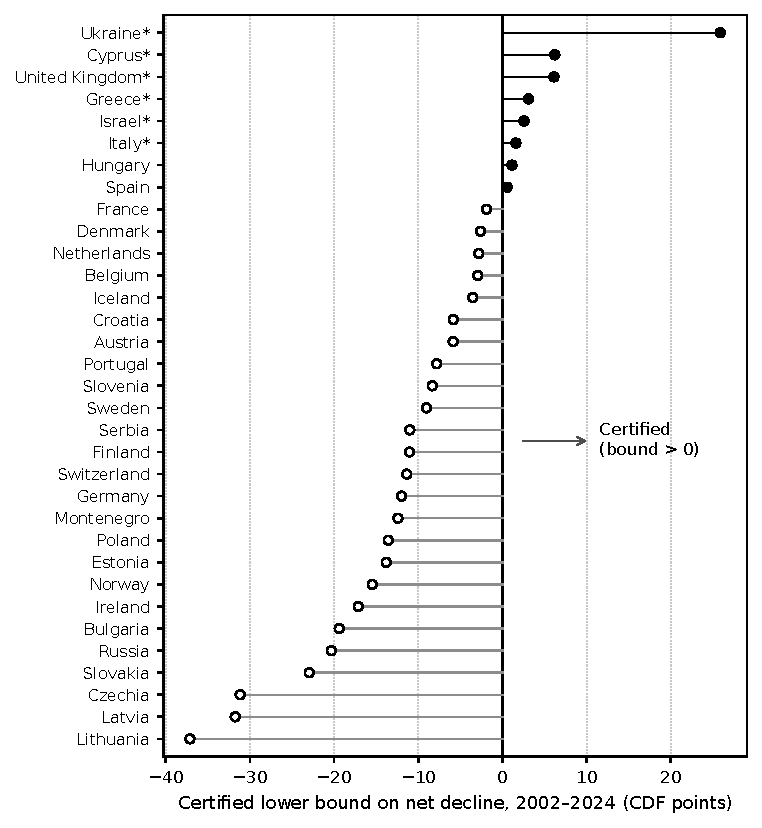
\includegraphics[width=.8\textwidth]{ess_net_bounds.pdf}
\caption{Each country's simultaneous lower bound on the net (first-to-last)
decline in parliamentary trust, 2002--2024, read off its joint band at
$\alpha=0.10$. Filled markers: the eight countries whose bound exceeds zero;
asterisks: the six named by the closed-testing prevalence bound. Negative
bounds say how far a country sits from certifying, not that it
improved.}\label{fig:bounds}
\end{figure}

The reclassified countries are the weak-signal, higher-noise cases---\emph{certified
by the marginal plug-in but inconclusive under the design-aware band}, never
``false positives,'' a term we reserve for simulation with known truth.

\paragraph{Two confounds this window cannot exclude.} Round-10 fieldwork
coincided with the pandemic's rally-round-the-flag movements, so ``persistent
decline through this window'' is a claim made against a rally; and nine
countries switched to self-completion at round 10, confounding wave-pair
shifts with mode effects, which no design bootstrap absorbs. A mode audit
from the data's own mode variable bounds it: the Greek pair is mode-constant
and net counts are unchanged when the switchers' confounded pairs are
excluded (Supplementary Material, with a preregistered age-group analysis
that finds no pooling artifact).

\paragraph{A second, global target: Foa--Mounk deconsolidation.} We preregistered a
reanalysis of the ``democratic deconsolidation'' thesis
\citep{foa2016democratic,foa2017signs} on the WVS/EVS trends (1981--2022,
$59$--$77$ countries with $\ge2$ waves), recoding the five-item battery so that
deconsolidation is a persistent decline over each scale's preregistered core.
The harmonized trend file provides no design metadata, so this is an external
substantive stress test of the thesis, not a second validation of the method;
the ESS carries the design-based validity story. The verdict is calibration,
not denial, but the surviving phenomenon is not the one the thesis was about.
A \emph{marginal wave-pair reading of the same data}, constructed to
instantiate the bottom rung, flags $36$--$64$ countries per item against
$6$--$17$ (8--24\%) at the persistent rung. That $2.6$--$6.5\times$ ratio compounds two
changes: holding the inference layer fixed, the rung alone accounts for
$1.7$--$4.8\times$ (plug-in) or $1.9$--$4.8\times$ (design-aware), and
propagating design uncertainty at fixed rung accounts for the remainder.
Three caveats. The trend file carries no PSU/stratum identifiers, so the
weights-only bootstrap omits within-PSU dependence (variance-inflating) and
stratification (variance-reducing); where the former dominates, as is usual,
certified counts are \emph{inflated}: at variance $\times1.5$ and
$\times2.0$ the certified core holds at $13$ and $12$ countries and the gap
widens to $3.0$--$8.3\times$, so the reported gap is then a lower bound. The
per-item lists
carry no across-country familywise control, so we aggregate to multi-item
co-certification before interpreting geography. And the certification sets
sit below the $K\ge94$ bound, so every WVS band uses the full-$\alpha$
anchors of Theorem~\ref{thm:safe}.

\paragraph{The certified core: where the surviving deconsolidation lives.}
Aggregating per-item certifications yields a positive characterization
(Figure~\ref{fig:core}): of $38$ countries certified on $\ge1$ item, $13$
form a certified core on $\ge2$, headed by Albania on four. The core is
post-communist and Arab-Spring states, not the mature democracies the thesis
concerned,
formalizing with per-country error control the decline-from-euphoric-baselines
pattern the post-communist literature described qualitatively
\citep{mishler1997trajectories,inglehart2003honeymoon}. Three qualifications
travel with it. Five core members are electoral autocracies in the V-Dem
classification, where falling stated support reflects autocratic legitimation
rather than deconsolidation in the consolidated-democracy sense. The West enters
the core exactly twice (Finland and Switzerland, on the strongman/army pair,
which we flag as a probable administration artifact): no consolidated Western
democracy certifies on support for a democratic system, consistent with
\citet{wuttke2022europeans}, though not that the West is absent. And the
geography is partly window-contingent: recertifying on fieldwork ending by
2017 keeps eight of the thirteen but drops all three Arab-Spring cases, so
the post-communist component is window-stable and the Arab-Spring component
rests on WVS wave~7. Certified attitudes do not forecast institutions (core
membership predicts subsequent V-Dem electoral-democracy decline no better
than the marginal flag, Fisher $p=0.89$, a comparison too small to establish
the decoupling recent panel work expects,
\citealp{ouattara2023distrusting,vandermeer2025pushing}): certification is
descriptive error control, not a forecast (item-level caveats in the
Supplementary Material).

\begin{figure}[t]\centering
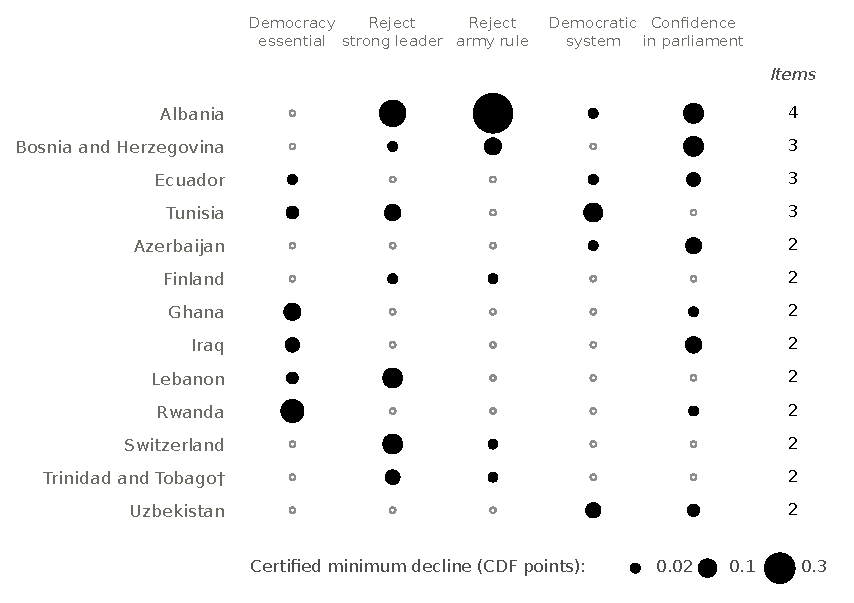
\includegraphics[width=.95\textwidth]{certified_core.pdf}
\caption{The thirteen-country certified core, by evidence strength (WVS/EVS
1981--2022; $K=59$--$77$ per item). Circle area is the persistent band's
simultaneous lower bound on the per-pair decline, in CDF points; open circles
mark items that do not certify. The full thirty-eight-country matrix is in the
Supplementary Material.}\label{fig:core}
\end{figure}

\section{Discussion}\label{sec:discussion}

Uncertainty in claims about repeated cross-national surveys is usually
computed for the wrong unit, twice. We have given a multiplicity-free
simultaneous band for the claim unit and a hard boundary for the calibration unit: the correction is
non-identified without the design-noise law (Theorem~\ref{thm:impossible}),
and unreachable for the deployed procedure at cross-national scale even with
it (Proposition~\ref{prop:unreach}). At the national unit the method reduces
to clustered population conformal, and the reported design share certifies
that the simple band is the right one. The deconvolution regime needs many
exchangeable units and comparable design noise, never both across countries
but reachable one unit down (Section~\ref{sec:evidence}).

\paragraph{Limitations.} The machinery prices sampling error only: measurement non-invariance
(wording changes, house effects, mode switches) produces the very shifts the
bands certify, so certifications straddling such changes are conditional on
measurement constancy. The
deployed $m$-of-$m$ PSU bootstrap \citep{rao1992recent,wolter2007introduction}
biases design variance downward; the Rao--Wu--Yue rescaled rerun leaves every
certification count and cross-national gate unchanged, while the small-area
activation set is bootstrap-sensitive in the disclosed direction
(Supplementary Material). Transport-band exchangeability is a
superpopulation postulate over a non-sampled, panel-attriting country set,
and holds worse for the post-communist bloc. And without design metadata
(the WVS trend file) only weights-only replication is possible.

\paragraph{The general lesson.} Attaching uncertainty to the right unit
changes substantive conclusions: no persistent decline certified among
thirty-three ESS countries over the full record, yet span erosion certified
in eight, mostly invisible to adjacent-wave readings; a certified
deconsolidation set several-fold smaller, concentrated outside the
consolidated West. The pattern is not confined to surveys: wherever prediction is calibrated on estimated objects
(Remark~\ref{rem:general}), the calibration targets carry their own error,
and the claim unit is often coarser than the trend asserted. The right
response is to state the strongest object the data support, correct
estimation noise where it is identified, and abstain where it is not, rather
than to widen every band reflexively.


% Flush any floats still pending (Figure 4 was landing after the references).
\clearpage

% PA specifies the order of the closing sections: Funding, Acknowledgements,
% Data Availability Statement, Competing Interests, figure legends, References.
\section*{Funding}
This research received no specific grant from any funding agency, commercial or
not-for-profit sector.

\section*{Acknowledgments}
From June through September 2026, the author used Claude Opus versions
4.8--5 via Claude.ai for limited assistance with figure preparation and
selected code implementation; it was not used to draft manuscript prose or
mathematical arguments. The author reviewed, executed, and verified all
AI-assisted material and takes full responsibility.

\section*{Data Availability Statement}
Replication code for this article is available at
\url{https://github.com/kunhailP/design-aware-conformal}; the package will be
deposited in the Political Analysis Dataverse with a version tag upon
conditional acceptance. Simulation, theory, and benchmark results are
deterministic under fixed seeds with no external data, and each theorem is
paired with an automated contract test checking its computational
implications. The survey microdata
\citep{essdata2024,wvsdata2024,lapopdata2023} are licensed to their providers
and cannot be redistributed; all code that runs on them is public, and the
replication package documents the exact file editions, variables, retrieval
steps, and sha256 checksums, alongside the public V-Dem and Claassen inputs
\citep{vdemdata2025,claassendata2020}. Three headline analyses have been
verified to reproduce the committed result tables bit-identically from the raw
licensed files in independent environments. The editor has been notified
of the restricted access at submission.

\section*{Competing Interests}
The author declares none.

\bibliographystyle{chicago}
\bibliography{refs}

\end{document}
